\documentclass{article}
\usepackage[margin=.9in]{geometry}
\usepackage{xcolor}
\usepackage{amsmath}
\usepackage{amssymb}
\usepackage{float}
\usepackage{listings}
\lstset{
  basicstyle=\small\ttfamily,
  breaklines=true,
  frame=single,
  language=Verilog,
  numbers=left,
  numberstyle=\tiny,
  showstringspaces=false
}
\setlength{\parindent}{0pt}
\setlength{\parskip}{\baselineskip}
\definecolor{mycolor}{rgb}{0.1, 0.1, 0.5}
\title{\textbf{{\huge Combinational Logic (Seven Segment Driver)}}}
\author{Christopher Hunt}
\date{}
\usepackage{graphicx} 
\usepackage{fancyhdr}

\begin{document}
\pagestyle{fancy}
\fancyhf{}
\rfoot{ENGR 272}
\lfoot{Christopher Hunt}
\lhead{Combinational Logic (Seven Segment Driver) }
\rhead{\thepage}
\maketitle
\section*{\textcolor{mycolor}{Objectives}}
The objective of this lab is to design and implement a decoder on the FPGA that can convert a 4-bit binary number inputted using the switches into a single digit of hexadecimal on the seven-segment display. This will be achieved by creating a block diagram for the decoder design, determining the mapping for displaying each number 0-F on the seven-segment display, generating the functional truth table for the decoder, minimizing the logic for each segment of the decoder using Karnaugh Maps, simulating the design, and finally programming and testing the hardware implementation on the DE10-Lite. Through this lab, we will learn about the process of designing and implementing a decoder, using Karnaugh Maps for logic minimization, and gaining hands-on experience with FPGA programming and testing.
\vspace{5mm}
\hrule

\section*{\textcolor{mycolor}{Equipment}}
\begin{itemize}
\item Quartus Prime Lite Edition V. 18.0
\item DE10-Lite kit with MAX10 10M50DAF484C7G FPGA
\item USB to USB-B cable
\end{itemize}
\vspace{5mm}
\hrule

\section*{\textcolor{mycolor}{Design}}
Our task is to display the hex digit which corresponds to a 4-bit binary number. First we must identify the segments which are on for each state. In figure one we have highlighted the output for each state.

\begin{figure}[H]
  \centering
  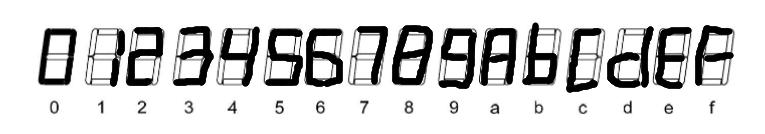
\includegraphics[width=1\textwidth]{digits.png}
  \caption{Digits to Hex}
\end{figure}

The next step in the design process is to map the inputs to the corresponding segement output. To accomplish that a truth table was constructed (Table 1).

% Truth Table 1
\begin{table}[H]
\centering
\begin{tabular}{|c|c|c|c|c|c|c|c|c|}
\hline
Hex & Input & Sa & Sb & Sc & Sd & Se & Sf & Sg \\
\hline
0 & 0000 & 0 & 0 & 0 & 0 & 0 & 0 & 1 \\
\hline
1 & 0001 & 1 & 0 & 0 & 1 & 1 & 1 & 1 \\
\hline
2 & 0010 & 0 & 0 & 1 & 0 & 0 & 1 & 0 \\
\hline
3 & 0011 & 0 & 0 & 0 & 0 & 1 & 1 & 0 \\
\hline
4 & 0100 & 1 & 0 & 0 & 1 & 1 & 0 & 0 \\
\hline
5 & 0101 & 0 & 1 & 0 & 0 & 1 & 0 & 0 \\
\hline
6 & 0110 & 0 & 1 & 0 & 0 & 0 & 0 & 0 \\
\hline
7 & 0111 & 0 & 0 & 0 & 1 & 1 & 1 & 1 \\
\hline
8 & 1000 & 0 & 0 & 0 & 0 & 0 & 0 & 0 \\
\hline
9 & 1001 & 0 & 0 & 0 & 0 & 1 & 0 & 0 \\
\hline
A & 1010 & 0 & 0 & 0 & 1 & 0 & 0 & 0 \\
\hline
b & 1011 & 1 & 1 & 0 & 0 & 0 & 0 & 0 \\
\hline
C & 1100 & 0 & 1 & 1 & 0 & 0 & 0 & 1 \\
\hline
d & 1101 & 1 & 0 & 0 & 0 & 0 & 1 & 0 \\
\hline
E & 1110 & 0 & 1 & 1 & 0 & 0 & 0 & 0 \\
\hline
F & 1111 & 0 & 1 & 1 & 1 & 0 & 0 & 0 \\
\hline
\end{tabular}
\caption{Input Switch to Output PIN Truth Table}
\end{table}

Considering that the 7-segment display pins are active LOW, we expect a value of 0 for the segments we want to be turned on during a particular state, while a value of 1 indicates that the segments should be turned off. To accomplish this, we generate Karnaugh maps for each possible output $S_a$ to $S_g$. These maps allow us to derive the boolean algebra expressions, which form the basis for our logic design (refer to Tables 4 through 8).

% Karnaugh Maps
% S_a and S_b
\begin{table}[H]
  \centering
  \begin{minipage}{0.45\textwidth}
  \centering
  \begin{tabular}{|c|c|c|c|c|}
  \hline
  \textbf{$D_3 \; D_2$} & \textbf{00} & \textbf{01} & \textbf{11} & \textbf{10} \\
  \hline
  \textbf{$D_1 \; D_0$} & | & | & | & | \\
  \hline
  \textbf{00} & 0 & 1 & 0 & 0 \\
  \hline
  \textbf{01} & 1 & 0 & 1 & 0 \\
  \hline
  \textbf{11} & 0 & 0 & 0 & 1 \\
  \hline
  \textbf{10} & 0 & 0 & 0 & 0 \\
  \hline
  \end{tabular}
  \caption{$S_a$ Karnaugh Map}
  \end{minipage}
  \hfill
  \begin{minipage}{0.45\textwidth}
  \centering
  \begin{tabular}{|c|c|c|c|c|}
  \hline
  \textbf{$D_3 \; D_2$} & \textbf{00} & \textbf{01} & \textbf{11} & \textbf{10} \\
  \hline
  \textbf{$D_1 \; D_0$} & | & | & | & | \\
  \hline
  \textbf{00} & 0 & 0 & 1 & 0 \\
  \hline
  \textbf{01} & 0 & 1 & 0 & 0 \\
  \hline
  \textbf{11} & 0 & 0 & 1 & 1 \\
  \hline
  \textbf{10} & 0 & 1 & 1 & 0 \\
  \hline
  \end{tabular}
  \caption{$S_b$ Karnaugh Map}
  \end{minipage}
\end{table}
\begin{align*}
  S_a =& \bar{D_3}\bar{D_2}\bar{D_1}D_0+\bar{D_3}D_2\bar{D_1}\bar{D_0}+D_3D_2\bar{D_1}D_0+D_3+\bar{D_2}D_1D_0\\
  S_b =&D_2D_1\bar{D_0}+D_3D_1D_0+D_3D_2\bar{D_0}+\bar{D_3}D_2\bar{D_1}D_0
\end{align*}


% S_c and S_d
\begin{table}[H]
  \centering
  \begin{minipage}{0.45\textwidth}
  \centering
  \begin{tabular}{|c|c|c|c|c|}
  \hline
  \textbf{$D_3 \; D_2$} & \textbf{00} & \textbf{01} & \textbf{11} & \textbf{10} \\
  \hline
  \textbf{$D_1 \; D_0$} & | & | & | & | \\
  \hline
  \textbf{00} & 0 & 0 & 1 & 0 \\
  \hline
  \textbf{01} & 0 & 0 & 0 & 0 \\
  \hline
  \textbf{11} & 0 & 0 & 1 & 0 \\
  \hline
  \textbf{10} & 1 & 0 & 1 & 0 \\
  \hline
  \end{tabular}
  \caption{$S_c$ Karnaugh Map}
  \end{minipage}
  \hfill
  \begin{minipage}{0.45\textwidth}
  \centering
  \begin{tabular}{|c|c|c|c|c|}
  \hline
  \textbf{$D_3 \; D_2$} & \textbf{00} & \textbf{01} & \textbf{11} & \textbf{10} \\
  \hline
  \textbf{$D_1 \; D_0$} & | & | & | & | \\
  \hline
  \textbf{00} & 0 & 1 & 0 & 0 \\
  \hline
  \textbf{01} & 1 & 0 & 0 & 0 \\
  \hline
  \textbf{11} & 0 & 1 & 1 & 0 \\
  \hline
  \textbf{10} & 0 & 0 & 0 & 1 \\
  \hline
  \end{tabular}
  \caption{$S_d$ Karnaugh Map}
  \end{minipage}
\end{table}
\begin{align*}
  S_c =& D_3D_2\bar{D_0}+D_3D_2D_1+\bar{D_3}\bar{D_2}D_1\bar{D_0}\\
  S_d =&D_2D_1D_0+\bar{D_3}\bar{D_2}\bar{D_1}D_0+\bar{D_3}D_2\bar{D_1}\bar{D_0}+D_3\bar{D_2}D_1\bar{D_0}
\end{align*}


% S_e and S_f
\begin{table}[H]
  \centering
  \begin{minipage}{0.45\textwidth}
  \centering
  \begin{tabular}{|c|c|c|c|c|}
  \hline
  \textbf{$D_3 \; D_2$} & \textbf{00} & \textbf{01} & \textbf{11} & \textbf{10} \\
  \hline
  \textbf{$D_1 \; D_0$} & | & | & | & | \\
  \hline
  \textbf{00} & 0 & 1 & 0 & 0 \\
  \hline
  \textbf{01} & 1 & 1 & 0 & 1 \\
  \hline
  \textbf{11} & 1 & 1 & 0 & 0 \\
  \hline
  \textbf{10} & 0 & 0 & 0 & 0 \\
  \hline
  \end{tabular}
  \caption{$S_e$ Karnaugh Map}
  \end{minipage}
  \hfill
  \begin{minipage}{0.45\textwidth}
  \centering
  \begin{tabular}{|c|c|c|c|c|}
  \hline
  \textbf{$D_3 \; D_2$} & \textbf{00} & \textbf{01} & \textbf{11} & \textbf{10} \\
  \hline
  \textbf{$D_1 \; D_0$} & | & | & | & | \\
  \hline
  \textbf{00} & 0 & 0 & 0 & 0 \\
  \hline
  \textbf{01} & 1 & 0 & 1 & 0 \\
  \hline
  \textbf{11} & 1 & 1 & 0 & 0 \\
  \hline
  \textbf{10} & 1 & 0 & 0 & 0 \\
  \hline
  \end{tabular}
  \caption{$S_f$ Karnaugh Map}
  \end{minipage}
\end{table}
\begin{align*}
  S_e =& \bar{D_2}\bar{D_1}D_0+\bar{D_3}D_2\bar{D_1}+\bar{D_3}D_2D_0+\bar{D_3}\bar{D_2}D_0\\
  S_f =& \bar{D_3}\bar{D_2}D_0+\bar{D_3}\bar{D_2}D_1+\bar{D_3}D_1D_0+D_3D_2\bar{D_1}D_0
\end{align*}

% S_g
\begin{table}[H]
\centering
\begin{tabular}{|c|c|c|c|c|}
\hline
\textbf{$D_3 \; D_2$} & \textbf{00} & \textbf{01} & \textbf{11} & \textbf{10} \\
\hline
\textbf{$D_1 \; D_0$} & | & | & | & | \\
\hline
\textbf{00} & 1 & 0 & 1 & 0 \\
\hline
\textbf{01} & 1 & 0 & 0 & 0 \\
\hline
\textbf{11} & 0 & 1 & 0 & 0 \\
\hline
\textbf{10} & 0 & 0 & 0 & 0 \\
\hline
\end{tabular}
\caption{$S_g$ Karnaugh Map}
\end{table}
\begin{equation*}
  S_g = \bar{D_3}\bar{D_2}\bar{D_1}+D_3D_2\bar{D_1}\bar{D_0}+\bar{D_3}D_2D_1D_0
\end{equation*}


\vspace{5mm}
\hrule

\subsection*{\textcolor{mycolor}{Design Entry}}
Once the boolean logic equations are derived, we utilize Quartus Prime to construct the schematics for each individual logic design (refer to figures 2 through 8). These schematics are then exported as symbol files and serve as logic blocks for the complete binary-to-hex digital display design (refer to figure 9). Subsequently, we proceed to FPGA pin placement, where the binary inputs are mapped to SW0 to SW2, and the display segments are mapped to their corresponding segments a through g (as illustrated in Table 9 and Table 10).
\begin{figure}[H]
  \centering
  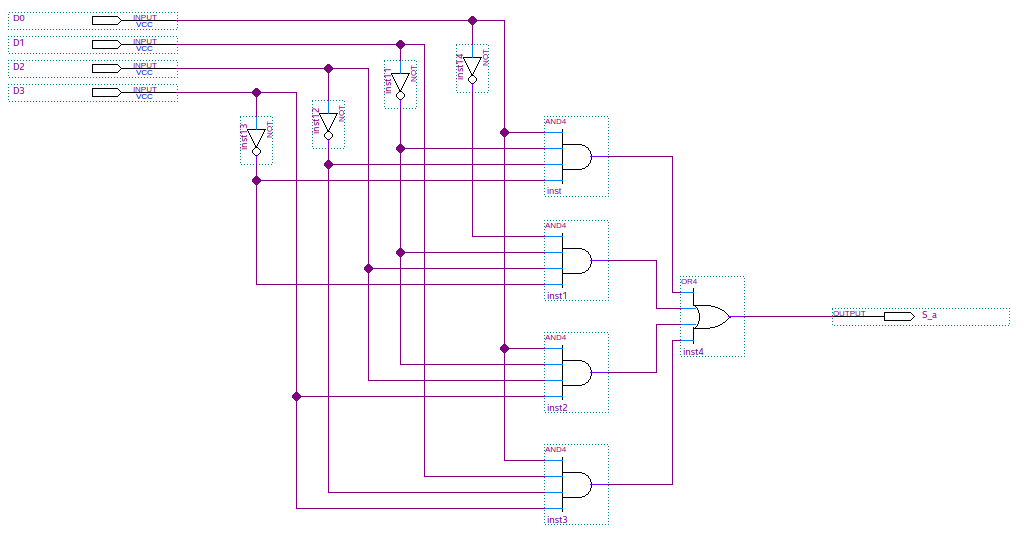
\includegraphics[width=1\textwidth]{S_a_schem.png}
  \caption{$S_a$ Digital Logic Schematic}
\end{figure}

\begin{figure}[H]
  \centering
  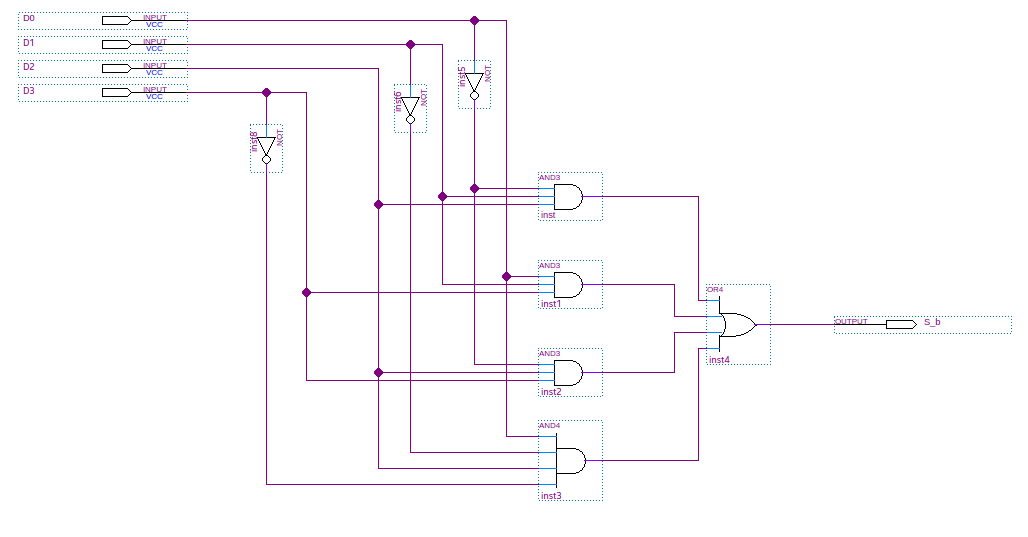
\includegraphics[width=1\textwidth]{S_b_schem.png}
  \caption{$S_b$ Digital Logic Schematic}
\end{figure}

\begin{figure}[H]
  \centering
  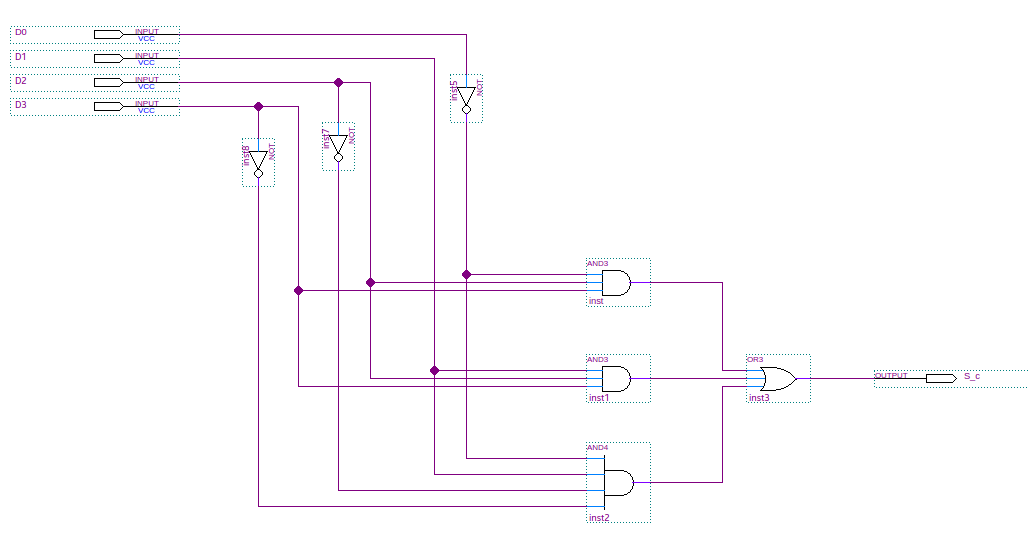
\includegraphics[width=1\textwidth]{S_c_schem.png}
  \caption{$S_c$ Digital Logic Schematic}
\end{figure}

\begin{figure}[H]
  \centering
  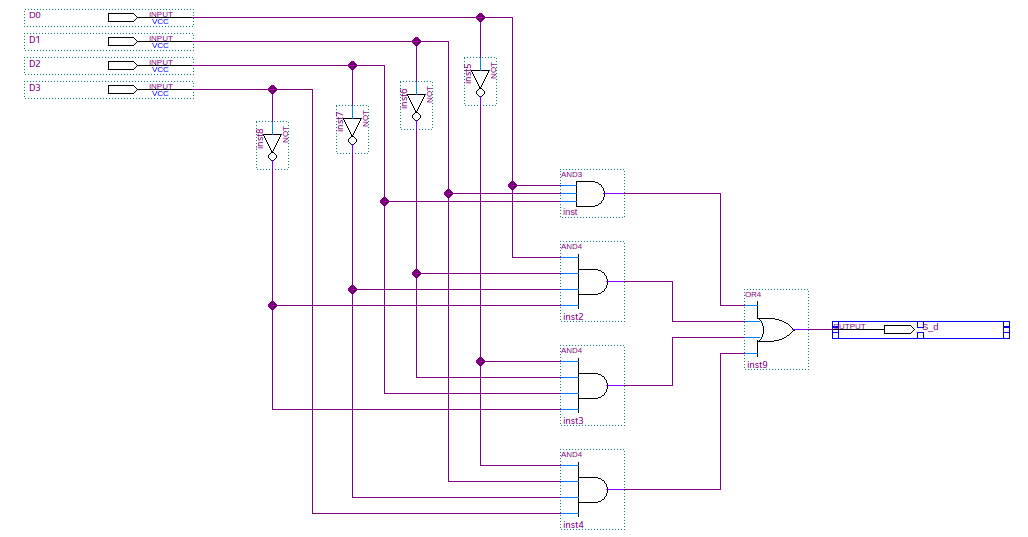
\includegraphics[width=1\textwidth]{S_d_schem.png}
  \caption{$S_e$ Digital Logic Schematic}
\end{figure}

\begin{figure}[H]
  \centering
  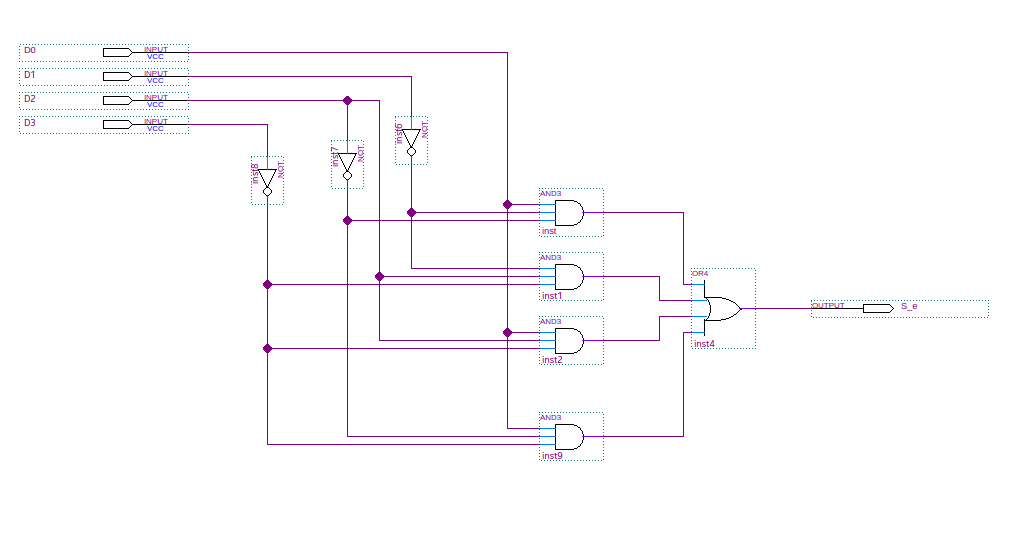
\includegraphics[width=1\textwidth]{S_e_schem.png}
  \caption{$S_f$ Digital Logic Schematic}
\end{figure}

\begin{figure}[H]
  \centering
  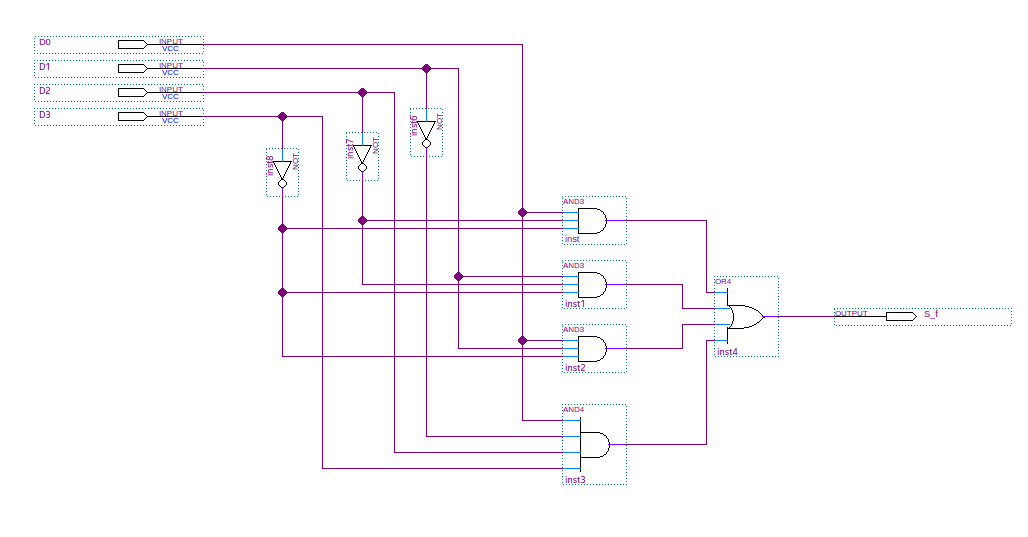
\includegraphics[width=1\textwidth]{S_f_schem.png}
  \caption{$S_g$ Digital Logic Schematic}
\end{figure}

\begin{figure}[H]
  \centering
  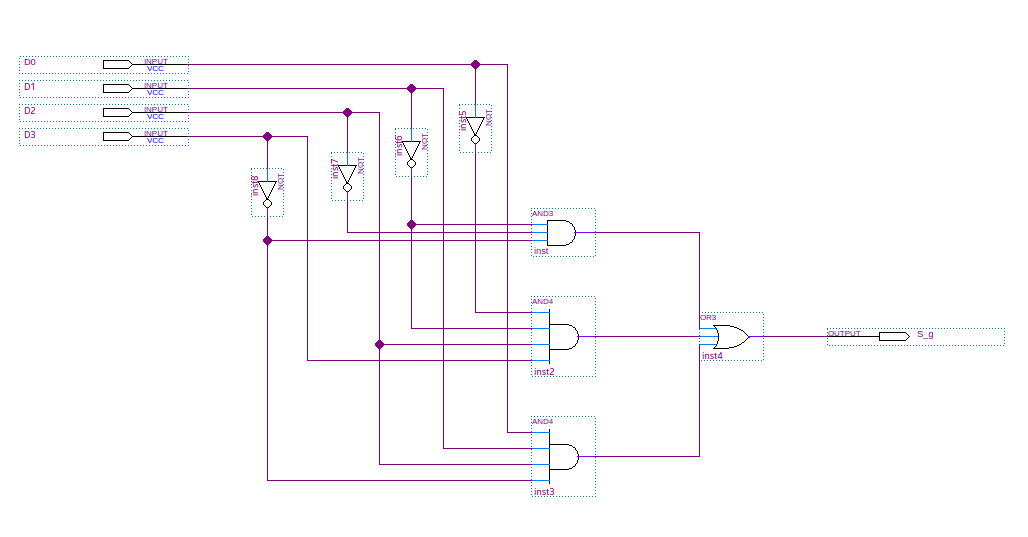
\includegraphics[width=1\textwidth]{S_g_schem.png}
  \caption{$S_g$ Digital Logic Schematic}
\end{figure}

\begin{figure}[H]
  \centering
  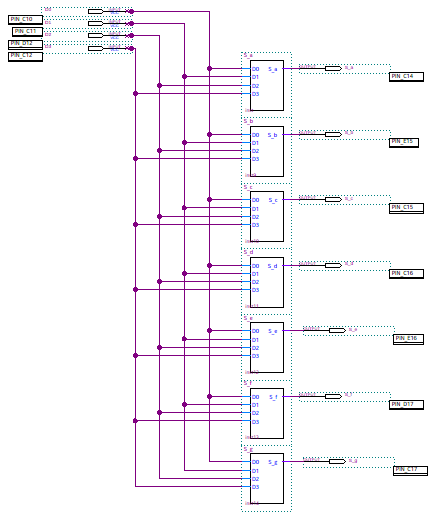
\includegraphics[width=.8\textwidth]{full_schem.png}
  \caption{Full Binary To Hex Display Digital Logic Schematic}
\end{figure}

% FPGA PIN Placement
\begin{table}[H]
\centering
\begin{minipage}{0.45\textwidth}
\centering
\begin{tabular}{|c|c|}
\hline
Input & FPGA PIN \\
\hline
D0 & PIN\_C10 \\ \hline
D1 & PIN\_C11 \\ \hline
D2 & PIN\_D12 \\ \hline
D3 & PIN\_C12 \\
\hline
\end{tabular}
\caption{Input to FPGA PIN Mapping}
\end{minipage}
\hfill
\begin{minipage}{0.45\textwidth}
\centering
\begin{tabular}{|c|c|}
\hline
Output & FPGA PIN \\
\hline
Sa & PIN\_C14 \\ \hline
Sb & PIN\_E15 \\ \hline
Sc & PIN\_C15 \\ \hline
Sd & PIN\_C16 \\ \hline
Se & PIN\_E16 \\ \hline
Sf & PIN\_D17 \\ \hline
Sg & PIN\_C17 \\
\hline
\end{tabular}
\caption{Output to FPGA PIN Mapping}
\end{minipage}
\end{table}
\vspace{5mm}
\hrule
\subsection*{\textcolor{mycolor}{Design Simulation}}
Simulation description, results table
\vspace{5mm}
\hrule

\section*{\textcolor{mycolor}{Design Implementation}}
Implementation description, results table, picture of implementation
\vspace{5mm}
\hrule

\section*{\textcolor{mycolor}{Observations}}
Observations of the lab
\vspace{5mm}
\hrule

\section*{\textcolor{mycolor}{Conclusion}}
In conclusion, the lab focused on the design and implementation of a decoder for converting a 4-bit binary number to a single digit of hexadecimal on a seven-segment display. Throughout the lab, various steps were undertaken to achieve this objective, including creating a block diagram, determining the display mapping, generating a functional truth table, minimizing the logic using Karnaugh Maps, simulating the design, and programming and testing the hardware on the FPGA.

By successfully completing the lab, we gained valuable knowledge and practical experience in designing digital logic circuits, using Karnaugh Maps for logic minimization, and programming FPGAs. We also developed an understanding of the relationship between binary numbers and their corresponding hexadecimal representation on a seven-segment display. This lab provided a hands-on opportunity to apply theoretical concepts and enhanced our skills in digital logic design and FPGA programming.

Overall, the lab helped deepen our understanding of combinational logic and its practical application in converting binary numbers to hexadecimal displays. It also highlighted the importance of careful design considerations, simulation, and hardware testing to ensure the desired functionality and accuracy of the implemented circuit.
\vspace{5mm}
\hrule

\section*{\textcolor{mycolor}{Study Questions}}
\subsubsection*{\textcolor{mycolor}{1. When is a simulation necessary? Was it useful for this section?}}


\end{document}